\documentclass[1p]{elsarticle_modified}
%\bibliographystyle{elsarticle-num}

%\usepackage[colorlinks]{hyperref}
%\usepackage{abbrmath_seonhwa} %\Abb, \Ascr, \Acal ,\Abf, \Afrak
\usepackage{amsfonts}
\usepackage{amssymb}
\usepackage{amsmath}
\usepackage{amsthm}
\usepackage{scalefnt}
\usepackage{amsbsy}
\usepackage{kotex}
\usepackage{caption}
\usepackage{subfig}
\usepackage{color}
\usepackage{graphicx}
\usepackage{xcolor} %% white, black, red, green, blue, cyan, magenta, yellow
\usepackage{float}
\usepackage{setspace}
\usepackage{hyperref}

\usepackage{tikz}
\usetikzlibrary{arrows}

\usepackage{multirow}
\usepackage{array} % fixed length table
\usepackage{hhline}

%%%%%%%%%%%%%%%%%%%%%
\makeatletter
\renewcommand*\env@matrix[1][\arraystretch]{%
	\edef\arraystretch{#1}%
	\hskip -\arraycolsep
	\let\@ifnextchar\new@ifnextchar
	\array{*\c@MaxMatrixCols c}}
\makeatother %https://tex.stackexchange.com/questions/14071/how-can-i-increase-the-line-spacing-in-a-matrix
%%%%%%%%%%%%%%%

\usepackage[normalem]{ulem}

\newcommand{\msout}[1]{\ifmmode\text{\sout{\ensuremath{#1}}}\else\sout{#1}\fi}
%SOURCE: \msout is \stkout macro in https://tex.stackexchange.com/questions/20609/strikeout-in-math-mode

\newcommand{\cancel}[1]{
	\ifmmode
	{\color{red}\msout{#1}}
	\else
	{\color{red}\sout{#1}}
	\fi
}

\newcommand{\add}[1]{
	{\color{blue}\uwave{#1}}
}

\newcommand{\replace}[2]{
	\ifmmode
	{\color{red}\msout{#1}}{\color{blue}\uwave{#2}}
	\else
	{\color{red}\sout{#1}}{\color{blue}\uwave{#2}}
	\fi
}

\newcommand{\Sol}{\mathcal{S}} %segment
\newcommand{\D}{D} %diagram
\newcommand{\A}{\mathcal{A}} %arc


%%%%%%%%%%%%%%%%%%%%%%%%%%%%%5 test

\def\sl{\operatorname{\textup{SL}}(2,\Cbb)}
\def\psl{\operatorname{\textup{PSL}}(2,\Cbb)}
\def\quan{\mkern 1mu \triangleright \mkern 1mu}

\theoremstyle{definition}
\newtheorem{thm}{Theorem}[section]
\newtheorem{prop}[thm]{Proposition}
\newtheorem{lem}[thm]{Lemma}
\newtheorem{ques}[thm]{Question}
\newtheorem{cor}[thm]{Corollary}
\newtheorem{defn}[thm]{Definition}
\newtheorem{exam}[thm]{Example}
\newtheorem{rmk}[thm]{Remark}
\newtheorem{alg}[thm]{Algorithm}

\newcommand{\I}{\sqrt{-1}}
\begin{document}

%\begin{frontmatter}
%
%\title{Boundary parabolic representations of knots up to 8 crossings}
%
%%% Group authors per affiliation:
%\author{Yunhi Cho} 
%\address{Department of Mathematics, University of Seoul, Seoul, Korea}
%\ead{yhcho@uos.ac.kr}
%
%
%\author{Seonhwa Kim} %\fnref{s_kim}}
%\address{Center for Geometry and Physics, Institute for Basic Science, Pohang, 37673, Korea}
%\ead{ryeona17@ibs.re.kr}
%
%\author{Hyuk Kim}
%\address{Department of Mathematical Sciences, Seoul National University, Seoul 08826, Korea}
%\ead{hyukkim@snu.ac.kr}
%
%\author{Seokbeom Yoon}
%\address{Department of Mathematical Sciences, Seoul National University, Seoul, 08826,  Korea}
%\ead{sbyoon15@snu.ac.kr}
%
%\begin{abstract}
%We find all boundary parabolic representation of knots up to 8 crossings.
%
%\end{abstract}
%\begin{keyword}
%    \MSC[2010] 57M25 
%\end{keyword}
%
%\end{frontmatter}

%\linenumbers
%\tableofcontents
%
\newcommand\colored[1]{\textcolor{white}{\rule[-0.35ex]{0.8em}{1.4ex}}\kern-0.8em\color{red} #1}%
%\newcommand\colored[1]{\textcolor{white}{ #1}\kern-2.17ex	\textcolor{white}{ #1}\kern-1.81ex	\textcolor{white}{ #1}\kern-2.15ex\color{red}#1	}

{\Large $\underline{11a_{243}~(K11a_{243})}$}

\setlength{\tabcolsep}{10pt}
\renewcommand{\arraystretch}{1.6}
\vspace{1cm}\begin{tabular}{m{100pt}>{\centering\arraybackslash}m{274pt}}
\multirow{5}{120pt}{
	\centering
	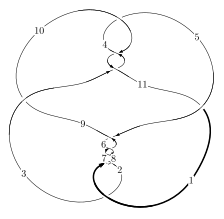
\includegraphics[width=112pt]{../../../GIT/diagram.site/Diagrams/png/492_11a_243.png}\\
\ \ \ A knot diagram\footnotemark}&
\allowdisplaybreaks
\textbf{Linearized knot diagam} \\
\cline{2-2}
 &
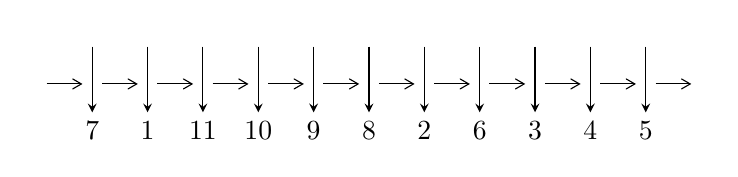
\begin{tikzpicture}[x=20pt, y=17pt]
	% nodes
	\node (C0) at (0, 0) {};
	\node (C1) at (1, 0) {};
	\node (C1U) at (1, +1) {};
	\node (C1D) at (1, -1) {7};

	\node (C2) at (2, 0) {};
	\node (C2U) at (2, +1) {};
	\node (C2D) at (2, -1) {1};

	\node (C3) at (3, 0) {};
	\node (C3U) at (3, +1) {};
	\node (C3D) at (3, -1) {11};

	\node (C4) at (4, 0) {};
	\node (C4U) at (4, +1) {};
	\node (C4D) at (4, -1) {10};

	\node (C5) at (5, 0) {};
	\node (C5U) at (5, +1) {};
	\node (C5D) at (5, -1) {9};

	\node (C6) at (6, 0) {};
	\node (C6U) at (6, +1) {};
	\node (C6D) at (6, -1) {8};

	\node (C7) at (7, 0) {};
	\node (C7U) at (7, +1) {};
	\node (C7D) at (7, -1) {2};

	\node (C8) at (8, 0) {};
	\node (C8U) at (8, +1) {};
	\node (C8D) at (8, -1) {6};

	\node (C9) at (9, 0) {};
	\node (C9U) at (9, +1) {};
	\node (C9D) at (9, -1) {3};

	\node (C10) at (10, 0) {};
	\node (C10U) at (10, +1) {};
	\node (C10D) at (10, -1) {4};

	\node (C11) at (11, 0) {};
	\node (C11U) at (11, +1) {};
	\node (C11D) at (11, -1) {5};
	\node (C12) at (12, 0) {};

	% arrows
	\draw[->,>={angle 60}]
	(C0) edge (C1) (C1) edge (C2) (C2) edge (C3) (C3) edge (C4) (C4) edge (C5) (C5) edge (C6) (C6) edge (C7) (C7) edge (C8) (C8) edge (C9) (C9) edge (C10) (C10) edge (C11) (C11) edge (C12) ;	\draw[->,>=stealth]
	(C1U) edge (C1D) (C2U) edge (C2D) (C3U) edge (C3D) (C4U) edge (C4D) (C5U) edge (C5D) (C6U) edge (C6D) (C7U) edge (C7D) (C8U) edge (C8D) (C9U) edge (C9D) (C10U) edge (C10D) (C11U) edge (C11D) ;
	\end{tikzpicture} \\
\hhline{~~} \\& 
\textbf{Solving Sequence} \\ \cline{2-2} 
 &
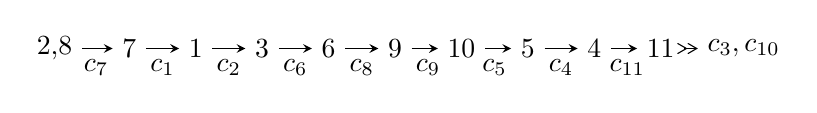
\begin{tikzpicture}[x=24pt, y=7pt]
	% node
	\node (A0) at (-1/8, 0) {2,8};
	\node (A1) at (1, 0) {7};
	\node (A2) at (2, 0) {1};
	\node (A3) at (3, 0) {3};
	\node (A4) at (4, 0) {6};
	\node (A5) at (5, 0) {9};
	\node (A6) at (6, 0) {10};
	\node (A7) at (7, 0) {5};
	\node (A8) at (8, 0) {4};
	\node (A9) at (9, 0) {11};
	\node (C1) at (1/2, -1) {$c_{7}$};
	\node (C2) at (3/2, -1) {$c_{1}$};
	\node (C3) at (5/2, -1) {$c_{2}$};
	\node (C4) at (7/2, -1) {$c_{6}$};
	\node (C5) at (9/2, -1) {$c_{8}$};
	\node (C6) at (11/2, -1) {$c_{9}$};
	\node (C7) at (13/2, -1) {$c_{5}$};
	\node (C8) at (15/2, -1) {$c_{4}$};
	\node (C9) at (17/2, -1) {$c_{11}$};
	\node (A10) at (41/4, 0) {$c_{3},c_{10}$};

	% edge
	\draw[->,>=stealth]	
	(A0) edge (A1) (A1) edge (A2) (A2) edge (A3) (A3) edge (A4) (A4) edge (A5) (A5) edge (A6) (A6) edge (A7) (A7) edge (A8) (A8) edge (A9) ;
	\draw[->>,>={angle 60}]	
	(A9) edge (A10);
\end{tikzpicture} \\ 

\end{tabular} \\

\footnotetext{
The image of knot diagram is generated by the software ``\textbf{Draw programme}" developed by Andrew Bartholomew(\url{http://www.layer8.co.uk/maths/draw/index.htm\#Running-draw}), where we modified some parts for our purpose(\url{https://github.com/CATsTAILs/LinksPainter}).
}\phantom \\ \newline 
\centering \textbf{Ideals for irreducible components\footnotemark of $X_{\text{par}}$} 
 
\begin{align*}
I^u_{1}&=\langle 
u^{34}+u^{33}+\cdots- u-1\rangle \\
\\
\end{align*}
\raggedright * 1 irreducible components of $\dim_{\mathbb{C}}=0$, with total 34 representations.\\
\footnotetext{All coefficients of polynomials are rational numbers. But the coefficients are sometimes approximated in decimal forms when there is not enough margin.}
\newpage
\renewcommand{\arraystretch}{1}
\centering \section*{I. $I^u_{1}= \langle u^{34}+u^{33}+\cdots- u-1 \rangle$}
\flushleft \textbf{(i) Arc colorings}\\
\begin{tabular}{m{7pt} m{180pt} m{7pt} m{180pt} }
\flushright $a_{2}=$&$\begin{pmatrix}0\\u\end{pmatrix}$ \\
\flushright $a_{8}=$&$\begin{pmatrix}1\\0\end{pmatrix}$ \\
\flushright $a_{7}=$&$\begin{pmatrix}1\\- u^2\end{pmatrix}$ \\
\flushright $a_{1}=$&$\begin{pmatrix}u\\- u^3+u\end{pmatrix}$ \\
\flushright $a_{3}=$&$\begin{pmatrix}- u^3\\u^5- u^3+u\end{pmatrix}$ \\
\flushright $a_{6}=$&$\begin{pmatrix}- u^2+1\\- u^2\end{pmatrix}$ \\
\flushright $a_{9}=$&$\begin{pmatrix}u^4- u^2+1\\u^4\end{pmatrix}$ \\
\flushright $a_{10}=$&$\begin{pmatrix}- u^{12}+u^{10}-3 u^8+2 u^6- u^2+1\\u^{14}-2 u^{12}+5 u^{10}-6 u^8+6 u^6-2 u^4+u^2\end{pmatrix}$ \\
\flushright $a_{5}=$&$\begin{pmatrix}- u^6+u^4-2 u^2+1\\- u^6- u^2\end{pmatrix}$ \\
\flushright $a_{4}=$&$\begin{pmatrix}- u^{32}+3 u^{30}+\cdots-4 u^2+1\\- u^{33}- u^{32}+\cdots+u+1\end{pmatrix}$ \\
\flushright $a_{11}=$&$\begin{pmatrix}- u^{15}+2 u^{13}-6 u^{11}+8 u^9-10 u^7+8 u^5-4 u^3+2 u\\- u^{15}+u^{13}-4 u^{11}+3 u^9-4 u^7+2 u^5-2 u^3+u\end{pmatrix}$\\ \flushright $a_{11}=$&$\begin{pmatrix}- u^{15}+2 u^{13}-6 u^{11}+8 u^9-10 u^7+8 u^5-4 u^3+2 u\\- u^{15}+u^{13}-4 u^{11}+3 u^9-4 u^7+2 u^5-2 u^3+u\end{pmatrix}$\\&\end{tabular}
\flushleft \textbf{(ii) Obstruction class $= -1$}\\~\\
\flushleft \textbf{(iii) Cusp Shapes $= 4 u^{33}-16 u^{31}-4 u^{30}+68 u^{29}+12 u^{28}-180 u^{27}-52 u^{26}+420 u^{25}+112 u^{24}-788 u^{23}-244 u^{22}+1248 u^{21}+376 u^{20}-1696 u^{19}-508 u^{18}+1916 u^{17}+528 u^{16}-1876 u^{15}-436 u^{14}+1504 u^{13}+248 u^{12}-1040 u^{11}-76 u^{10}+584 u^9-16 u^8-276 u^7+32 u^6+108 u^5-24 u^4-28 u^3+12 u^2+12 u-14$}\\~\\
\newpage\renewcommand{\arraystretch}{1}
\flushleft \textbf{(iv) u-Polynomials at the component}\newline \\
\begin{tabular}{m{50pt}|m{274pt}}
Crossings & \hspace{64pt}u-Polynomials at each crossing \\
\hline $$\begin{aligned}c_{1},c_{7}\end{aligned}$$&$\begin{aligned}
&u^{34}+u^{33}+\cdots- u-1
\end{aligned}$\\
\hline $$\begin{aligned}c_{2},c_{5},c_{6}\\c_{8}\end{aligned}$$&$\begin{aligned}
&u^{34}+7 u^{33}+\cdots+7 u+1
\end{aligned}$\\
\hline $$\begin{aligned}c_{3},c_{4},c_{10}\end{aligned}$$&$\begin{aligned}
&u^{34}- u^{33}+\cdots-3 u-1
\end{aligned}$\\
\hline $$\begin{aligned}c_{9},c_{11}\end{aligned}$$&$\begin{aligned}
&u^{34}+u^{33}+\cdots-11 u-2
\end{aligned}$\\
\hline
\end{tabular}\\~\\
\newpage\renewcommand{\arraystretch}{1}
\flushleft \textbf{(v) Riley Polynomials at the component}\newline \\
\begin{tabular}{m{50pt}|m{274pt}}
Crossings & \hspace{64pt}Riley Polynomials at each crossing \\
\hline $$\begin{aligned}c_{1},c_{7}\end{aligned}$$&$\begin{aligned}
&y^{34}-7 y^{33}+\cdots-7 y+1
\end{aligned}$\\
\hline $$\begin{aligned}c_{2},c_{5},c_{6}\\c_{8}\end{aligned}$$&$\begin{aligned}
&y^{34}+41 y^{33}+\cdots+y+1
\end{aligned}$\\
\hline $$\begin{aligned}c_{3},c_{4},c_{10}\end{aligned}$$&$\begin{aligned}
&y^{34}+29 y^{33}+\cdots-7 y+1
\end{aligned}$\\
\hline $$\begin{aligned}c_{9},c_{11}\end{aligned}$$&$\begin{aligned}
&y^{34}-15 y^{33}+\cdots-25 y+4
\end{aligned}$\\
\hline
\end{tabular}\\~\\
\newpage\flushleft \textbf{(vi) Complex Volumes and Cusp Shapes}
$$\begin{array}{c|c|c}  
\text{Solutions to }I^u_{1}& \I (\text{vol} + \sqrt{-1}CS) & \text{Cusp shape}\\
 \hline 
\begin{aligned}
u &= -0.747104 + 0.637416 I\end{aligned}
 & \phantom{-}6.64470 + 2.36489 I & -2.86883 - 3.72968 I \\ \hline\begin{aligned}
u &= -0.747104 - 0.637416 I\end{aligned}
 & \phantom{-}6.64470 - 2.36489 I & -2.86883 + 3.72968 I \\ \hline\begin{aligned}
u &= -0.899925 + 0.475897 I\end{aligned}
 & -2.14151 + 4.62376 I & -13.8382 - 7.0838 I \\ \hline\begin{aligned}
u &= -0.899925 - 0.475897 I\end{aligned}
 & -2.14151 - 4.62376 I & -13.8382 + 7.0838 I \\ \hline\begin{aligned}
u &= \phantom{-}0.872014 + 0.400496 I\end{aligned}
 & \phantom{-}0.949146 - 0.978585 I & -10.88963 + 3.28439 I \\ \hline\begin{aligned}
u &= \phantom{-}0.872014 - 0.400496 I\end{aligned}
 & \phantom{-}0.949146 + 0.978585 I & -10.88963 - 3.28439 I \\ \hline\begin{aligned}
u &= \phantom{-}0.922322 + 0.514518 I\end{aligned}
 & \phantom{-}2.40379 - 8.43362 I & -8.56504 + 8.66068 I \\ \hline\begin{aligned}
u &= \phantom{-}0.922322 - 0.514518 I\end{aligned}
 & \phantom{-}2.40379 + 8.43362 I & -8.56504 - 8.66068 I \\ \hline\begin{aligned}
u &= -0.911159 + 0.064557 I\end{aligned}
 & -0.80027 + 3.72913 I & -14.4528 - 4.1895 I \\ \hline\begin{aligned}
u &= -0.911159 - 0.064557 I\end{aligned}
 & -0.80027 - 3.72913 I & -14.4528 + 4.1895 I \\ \hline\begin{aligned}
u &= \phantom{-}0.901185\phantom{ +0.000000I}\end{aligned}
 & -4.70685\phantom{ +0.000000I} & -19.4900\phantom{ +0.000000I} \\ \hline\begin{aligned}
u &= \phantom{-}0.703635 + 0.475487 I\end{aligned}
 & \phantom{-}1.07563 - 1.83024 I & -6.47079 + 5.97936 I \\ \hline\begin{aligned}
u &= \phantom{-}0.703635 - 0.475487 I\end{aligned}
 & \phantom{-}1.07563 + 1.83024 I & -6.47079 - 5.97936 I \\ \hline\begin{aligned}
u &= \phantom{-}0.484387 + 0.660768 I\end{aligned}
 & \phantom{-}3.79773 + 4.05189 I & -4.65777 - 2.65947 I \\ \hline\begin{aligned}
u &= \phantom{-}0.484387 - 0.660768 I\end{aligned}
 & \phantom{-}3.79773 - 4.05189 I & -4.65777 + 2.65947 I \\ \hline\begin{aligned}
u &= -0.905647 + 0.876658 I\end{aligned}
 & \phantom{-}8.74108 + 3.00465 I & -6.23462 - 3.51022 I \\ \hline\begin{aligned}
u &= -0.905647 - 0.876658 I\end{aligned}
 & \phantom{-}8.74108 - 3.00465 I & -6.23462 + 3.51022 I \\ \hline\begin{aligned}
u &= \phantom{-}0.887193 + 0.895874 I\end{aligned}
 & \phantom{-}6.61353 + 1.01180 I & -9.12967 - 1.18783 I \\ \hline\begin{aligned}
u &= \phantom{-}0.887193 - 0.895874 I\end{aligned}
 & \phantom{-}6.61353 - 1.01180 I & -9.12967 + 1.18783 I \\ \hline\begin{aligned}
u &= -0.885998 + 0.911204 I\end{aligned}
 & \phantom{-}11.67770 - 4.89843 I & -4.67803 + 2.35929 I \\ \hline\begin{aligned}
u &= -0.885998 - 0.911204 I\end{aligned}
 & \phantom{-}11.67770 + 4.89843 I & -4.67803 - 2.35929 I \\ \hline\begin{aligned}
u &= -0.933946 + 0.863515 I\end{aligned}
 & \phantom{-}8.64990 + 3.44136 I & -6.50419 - 1.50666 I \\ \hline\begin{aligned}
u &= -0.933946 - 0.863515 I\end{aligned}
 & \phantom{-}8.64990 - 3.44136 I & -6.50419 + 1.50666 I \\ \hline\begin{aligned}
u &= -0.440591 + 0.564184 I\end{aligned}
 & -0.754026 - 0.647677 I & -10.09307 + 0.88782 I \\ \hline\begin{aligned}
u &= -0.440591 - 0.564184 I\end{aligned}
 & -0.754026 + 0.647677 I & -10.09307 - 0.88782 I \\ \hline\begin{aligned}
u &= \phantom{-}0.957008 + 0.864633 I\end{aligned}
 & \phantom{-}6.39073 - 7.51888 I & -9.58479 + 5.88933 I \\ \hline\begin{aligned}
u &= \phantom{-}0.957008 - 0.864633 I\end{aligned}
 & \phantom{-}6.39073 + 7.51888 I & -9.58479 - 5.88933 I \\ \hline\begin{aligned}
u &= \phantom{-}0.933149 + 0.900837 I\end{aligned}
 & \phantom{-}15.8663 - 3.3207 I & -2.12280 + 2.39131 I \\ \hline\begin{aligned}
u &= \phantom{-}0.933149 - 0.900837 I\end{aligned}
 & \phantom{-}15.8663 + 3.3207 I & -2.12280 - 2.39131 I \\ \hline\begin{aligned}
u &= -0.967526 + 0.871929 I\end{aligned}
 & \phantom{-}11.4151 + 11.4767 I & -5.20067 - 7.04203 I\\
 \hline 
 \end{array}$$\newpage$$\begin{array}{c|c|c}  
\text{Solutions to }I^u_{1}& \I (\text{vol} + \sqrt{-1}CS) & \text{Cusp shape}\\
 \hline 
\begin{aligned}
u &= -0.967526 - 0.871929 I\end{aligned}
 & \phantom{-}11.4151 - 11.4767 I & -5.20067 + 7.04203 I \\ \hline\begin{aligned}
u &= \phantom{-}0.226712 + 0.537212 I\end{aligned}
 & \phantom{-}2.73574 - 2.31248 I & -4.68504 + 3.18940 I \\ \hline\begin{aligned}
u &= \phantom{-}0.226712 - 0.537212 I\end{aligned}
 & \phantom{-}2.73574 + 2.31248 I & -4.68504 - 3.18940 I \\ \hline\begin{aligned}
u &= -0.490234\phantom{ +0.000000I}\end{aligned}
 & -0.620230\phantom{ +0.000000I} & -16.5580\phantom{ +0.000000I}\\
 \hline 
 \end{array}$$\newpage
\newpage\renewcommand{\arraystretch}{1}
\centering \section*{ II. u-Polynomials}
\begin{tabular}{m{50pt}|m{274pt}}
Crossings & \hspace{64pt}u-Polynomials at each crossing \\
\hline $$\begin{aligned}c_{1},c_{7}\end{aligned}$$&$\begin{aligned}
&u^{34}+u^{33}+\cdots- u-1
\end{aligned}$\\
\hline $$\begin{aligned}c_{2},c_{5},c_{6}\\c_{8}\end{aligned}$$&$\begin{aligned}
&u^{34}+7 u^{33}+\cdots+7 u+1
\end{aligned}$\\
\hline $$\begin{aligned}c_{3},c_{4},c_{10}\end{aligned}$$&$\begin{aligned}
&u^{34}- u^{33}+\cdots-3 u-1
\end{aligned}$\\
\hline $$\begin{aligned}c_{9},c_{11}\end{aligned}$$&$\begin{aligned}
&u^{34}+u^{33}+\cdots-11 u-2
\end{aligned}$\\
\hline
\end{tabular}\newpage\renewcommand{\arraystretch}{1}
\centering \section*{ III. Riley Polynomials}
\begin{tabular}{m{50pt}|m{274pt}}
Crossings & \hspace{64pt}Riley Polynomials at each crossing \\
\hline $$\begin{aligned}c_{1},c_{7}\end{aligned}$$&$\begin{aligned}
&y^{34}-7 y^{33}+\cdots-7 y+1
\end{aligned}$\\
\hline $$\begin{aligned}c_{2},c_{5},c_{6}\\c_{8}\end{aligned}$$&$\begin{aligned}
&y^{34}+41 y^{33}+\cdots+y+1
\end{aligned}$\\
\hline $$\begin{aligned}c_{3},c_{4},c_{10}\end{aligned}$$&$\begin{aligned}
&y^{34}+29 y^{33}+\cdots-7 y+1
\end{aligned}$\\
\hline $$\begin{aligned}c_{9},c_{11}\end{aligned}$$&$\begin{aligned}
&y^{34}-15 y^{33}+\cdots-25 y+4
\end{aligned}$\\
\hline
\end{tabular}
\vskip 2pc
\end{document}